\section{Work Done}
The flow of the system and the various components are discussed, which is followed by the description of work done. 
\begin{figure}[!htb]
\centering
\includegraphics[scale=0.5]{figs/flow_b_w.eps}
\caption{Overall Flow of Mobility Summary Framework}
\label{fig:components}
\end{figure}

Figure \ref{fig:components} shows the different components for computing the \emph{mobility summary}, which in turn can be used for a variety of applications that rely on frequent-mobility based queries.The various components of the framework are described briefly below: 

%% 1 Trajectory Segmentation
%% 2. Trajectory Similarity
%% 3. Clustering
%% 
\begin{itemize}
\item{\emph{Input:}}
The input is in the form of a raw collection of three tuples, which are the \emph{location traces} of the person or user.
\item{\textbf{Preprocessing:}} 
Preprocessing module consists of the steps segmentation and normalization. Segmentation is the process of deciphering meaningful trips out of the raw traces. The second component is normalization, where each of the points is normalized according to the extents of latitude and longitude values.
\item{\textbf{Trajectory Similarity:}}
This is the module which defines and computes the similarity between all the pairs of trajectories in the dataset. This is a very crucial step as the clustering depends on the goodness of the similarity measure.
\item{\textbf{Trajectory Clustering:}} 
This module takes as input the similarity matrix formed in the earlier step, and runs a clustering algorithm on it and outputs a final cluster of trajectories. This step also encompasses outlier or anomaly detection.
\item{\textbf{Representative Trajectory:}} 
One trajectory per cluster which can act as the representative trajectory for that cluster needs to be computed for each of the final clusters. This task is taken up in this section.
\item{\textbf{Applications:}}
The applications of \emph{movement summary} include next path prediction and anomaly detection. Next path prediction is predicting the next path or destination of a given query trajectory based on the user's mobility history. Anomaly detection deals with recognizing anomalous behaviour of the user and classifying the query trajectory accordingly.
\end{itemize}

\subsection{Trajectory Preprocessing} 

\paragraph{Segmentation:}
The first step in preprocessing is to identify meaningful trips of a user using trajectory segmentation approaches~\cite{Zheng2008}. The input to the module is a raw file of three tuples containing the latitude and longitude of the user sampled at various time instances. This does not necessarily consist of moving trajectories, it might also contain tuples where the user is static for a long time. The aim is to eliminate such tuples, and extract only the meaningful trajectories where the user is in motion or has made a trip. Here the distance, velocity and time-gap between consecutive set of sample points are computed to identify if the user is mobile. The well-known representation of trajectory to denote a meaningful trip is used; it is an ordered set of 3-tuples $\langle \operatorname{latitude},\operatorname{longitude},\operatorname{time} \rangle$.
\paragraph{Normalization:}
The next step is to normalize the user locations since small changes in latitude and longitude can result in large distances on earth. Each raw latitude $\rawlat_i$ in the sample is normalized into a normalized latitude $\lat_i$ in the range $[0,1]$ as:
\begin{eqnarray}
\lat_i =\frac{\rawlat_i - \minlat}{\maxlat - \minlat}
\end{eqnarray}
where $\minlat=\min(\rawlat_j, \forall j)$ is the minimum latitude observed, and $\maxlat=\max(\rawlat_j, \forall j)$. 

Similarly, the raw longitude $\rawlon_i$ in converted to a normalized longitude $\lon_i$ in the range $[0,1]$ as:
\begin{eqnarray}
\lon_i =\frac{\rawlon_i - \minlon}{\maxlon - \minlon}
\end{eqnarray}
where $\minlon=\min(\rawlon_j, \forall j)$ is the minimum longitude observed, and $\maxlon=\max(\rawlon_j, \forall j)$. 


\subsection{Trajectory Similarity Analysis}

Computing the distance between a pair of trajectories is crucial to finding \emph{movement summaries} because higher level clustering algorithms require such a distance measure. A large number of trajectory similarity metrics, which give an estimate of the trajectory distance, have been proposed for various types of applications. Standard LP-Norm and ERP have been shown to be metrics~\cite{Chen2004}, where as a large number of other heuristic measures (such as LCSS, DTW, EDR) are non-metrics~\cite{Vlachos2002,Yi1998,Chen2005}. 
%A taxonomy of trajectory similarity metrics is discussed in Table~\ref{tab:simTaxonomy}. 
%\begin{table*}
%	\centering
%	\resizebox{\textwidth}{!}{
%		\begin{tabular}{|c|c|c|c|c|c|} 
%			\hline
%			Sim Measure&Is Metric&Type&Sen. to sample noise&OD Cognizant&Computational Cost\\
%			\hline
%			LP Norm&Yes&Sampling Sensitive&No&No&O(N)\\
%			DTW/LCSS/EDW/EDW With real sequences&No&Sampling Sensitive&Yes&No&O($n^2$)\\
%%			EDWP&Yes&Sampling Sensitive&Yes&No&??\\
%			LP Norm with Interpolation&Yes&Shape Sensitive&No&No&O(Num samples)\\
%			ODSim (Ours)&Yes&Shape sensitive&No&No&O(Num samples)\\
%			\hline
%		\end{tabular}}
%	\caption{Taxonomy of Similarity Measures}
%	\label{tab:simTaxonomy}
%\end{table*}

%The table talks about various features of a similarity function described as follows:\\
%Is Metric:It is important for a similarity measure to be mathematical metric. The conditions for being a mathematical metric are it should be symmetric, values should be non-negative, and it should follow triangle inequality. If a similarity measure is not a metric, problems might come up while clustering based on the similarity matrix. \\
%Type: Sampling sensitive measures vary hugely on the way the data points are sampled and the time interval at which they are sampled. Shape sensitive measures give more importance to the shape of the trajectory than the sample points, thus making it more robust.\\
%Sensitive to sampling noise\\
%Origin-Destination Cognizant : As the mobility summary is defined for human movement, it would be an advantage if the similarity measure is Origin-Destination cognizant.\\
%Computation Cost.\\

Non-metric distance functions are clearly inappropriate in clustering. In addition, it is shown that blindly using the existing non-metric distance functions not only result in sub-optimal clusters but also incur significant high cost in terms of computational time. A primary reason for the most non-metric functions (LCSS, DTW, EDR, ERP) are designed to suppress noise using techniques such as dynamic programming. However, for GPS trajectory, de-noising can be done as a preprocessing step, by removing or resampling the outlier points~\cite{Yuan2013,Zheng2009}. Hence, the modified standard LP-Norm functions are used for distance computation, avoiding time consuming non-metric algorithms.

\subsubsection{Curve Distance for Trajectories}
Instead of treating trajectory as a set of sample points, the trajectories can be approximated as curves on n-dimensional vector space. This approximation is reasonable if the location traces contain finely sampled GPS points (as in this case)%\rednote{Need more justification and some defense here. Basically, if not LP-Norm will work too}. 

%\rednote{Vinay: Karthik, please improve the below gibberish. I have taken the representation from Sebastien's paper}
For trajectory representation, the main idea is to represent a trajectory as a curve in two independent dimensions latitude and longitude (in $\mathbb{R}^2$)~\cite{Kurtek2012}. A natural extension is to represent in three independent dimensions including time. However, in this work, only latitude and longitude dimensions are looked into. %\rednote{Why are we ignoring time? We dont know how to weigh time and space together while measuring distances}. 

Let $f_i[0,1] \rightarrow \mathbb{R}^2$ be the curve for the $\operatorname{i}$-th trajectory trajectory, which maps a number between 0 to 1 to the (latitude, longitude) pairs of the trajectory. The standard $\mathbb{L}^2$ norm for this curve is given $\norm{f_i} = \left[ \int_{0}^{1}{f_i(x)^2\, \mathrm{d}x }\right] ^ {\frac{1}{2}}$. %\rednote{Karthik: Please correct this. How does the next sentence fall out from the prev definitions?} With this notion, the Curve Distance (CD) between two trajectories $t_i$ and $t_j$ is given by the $\mathbb{L}^2$ distance:
\begin{align}
\LP(t_i,t_j) = \left[ \int_{0}^{1}{\left(f_i(x) - f_j(x) \right )^2\, \mathrm{d}x }\right] ^ {\frac{1}{2}}.
\end{align}

Numerically, this is solved by first resampling the trajectory to a large number of points for each trajectory (100 samples in our case) and then using Trapezoidal Rule to find the curve distance. %\rednote{Vinay: Karthik, Can you fill a good refernce for trapezoidal rule}.

\paragraph{Weighted Curve Distance} For human mobility, a user's meaningful trip has an associated intention (such as commuting to work or grocery shop visit). More often, each frequent trajectory is between end-points that are important to the user (such as home and work). A metric is hence proposed that emphasizes origin and destination of the trajectories, while computing the distance. 

At first, the Curve Distance is generalized to Weighted Curve Distance, where all trajectories have different weights at each point.  It can be shown that the Weighted Curve Distance (WCD) between two trajectories $t_i$ and $t_j$ is given by
\begin{align}
\weightLP(t_i,t_j) = \left[ \int_{0}^{1}{ w(x) \left( f_i(x) - f_j(x) \right )^2\, \mathrm{d}x }\right] ^ {\frac{1}{2}}.
\end{align}
\noindent where $w(x) \rightarrow [0,1]$ is a weighting function. In the case of providing higher weights to origin and destination an Origin-Destination (OD) weighting function should be constructed such that the weights are high at the ends than at the center. We use Beta function $\operatorname{B(\alpha,\alpha)}$, where $\alpha$ in $[0,1]$. This provides a bimodal curve where weights at the ends are higher than the weights at the intermediate points in the curve; lower values of alpha provide very high values at ends than at the intermediate points.

Since CD is a metric and WCD is a weighted combination of CD (with positive weights), it can be shown that WCD is also a metric.

%\rednote{Vinay: Karthik, please comment}. 



%\rednote{$===================$Karthik Checkpoint end$===================$}
\subsection{Trajectory Clustering}
The distance matrices are used to aggregate similar trajectories into one cluster. Hierarchical agglomerative clustering is used since it provides the flexibility of analyzing the entire merge history of user's trajectories, and then cutting the dendrogram at the right level. This enables to personalize and automate clusters for different users. Each user has different motion patterns and -- apriori -- no information of how often/densely a user travels along different paths is known. The proposed system automatically recognizes the right number of clusters by analyzing the dendrogram.

Average link clustering is used to measure similarity between intermediate clusters. This is to avoid bias for clustering trajectories that are associatively near (using single-link) or by concentrating on the extreme points of the merge (using complete-link).%\rednote{Explain clearly. Show that complete or single has problems. Then say that DBSCAN also has problems. More probably so if single-link does not give good results}
\begin{algorithm}
\KwIn{Dendrogram with cluster information at each level}
\KwOut{Optimal Clusters (Trip Summaries)}    

\SetAlgoLined
\SetKwFunction{isSummary}{isSummary}
\For{\text{k=1 to N}}
{
\begin{equation}
SSW(Clus_i)= \sum_{j=1}^{|Trajs(Clus_i)|}{(Sim(Traj_{j},Mean(Clus_i)))^{2}}
\end{equation}
\begin{equation}
SSW(Level_k)=\sum_{j=1}^{k}{SSW(Cluster_j)}
\end{equation}
}
Find the elbow point from the SSW Plot over all levels \\
Set all trajectories as \textit{unmarked}\\
\For{\text{k=elbowPoint+1 to N}}
{
\For{\text{Each non anomalous  cluster}}
{
\If{Trajs(Cluster) are unmarked \&\& \isSummary{$Cluster_i$} }
{
Report Cluster as a final Cluster\\
Mark all Trajs in Cluster
}
}
}
\isSummary{$Cluster_i$}{

\For{All pairs of trajectories in Cluster}
{
 \If{Maximum Pointwise Distance$\le$ $\delta$  (kms)}
 {
\KwRet True}
}
\KwRet False
}
\\

\caption{Algorithm for reporting final clusters from Dendrogram}

\end{algorithm}
\subsubsection{Finding optimal clusters}
In this step, the dendrogram is cut at a level that defines meaningful mobility clusters. The main idea is to determine the optimal number of clusters for each person, and to use that knowledge to cut the dendrogram. A static similarity level to cut dendrogram is not chosen since different people have different forms of mobility. A user whose main travel pattern is long distance commute to two office locations has different distance thresholds than a student who is commuting mainly commuting from dormitory to classes. 

Existing well-known methods, such as the elbow method, do not cut the dendogram at appropriate level to provide good movement summaries; which is demonstrated in Section $4.4$. Hence, an algorithm is designed that cuts the dendogram at a level where trajectories in a cluster are between nearby origin and destinations, which signify similar meaningful trips of a person.
%\newenvironment{badidea}
%  {\par\leftskip=2cm}
%  {\par}


%\rednote{Vinay: Manasa, can you please insert the algorithm (in latex algorithmic style)}

The algorithm iterates down the dendrogram starting at the root; the number of clusters at this stage being $k=1$ . As we proceed down each level to cut the dendrogram, the number of clusters $k$ increases by one. We compute the possible summary clusters of the user for each $k$. Let $\setSummClus_k =  \{ \summClus_{ki}, \forall i \}$ be the set of clusters for the user at level $k$. Let $t_{kij}$ be the $\operatorname{j}$-th trajectory in $\summClus_{ki}$. Let the mean trajectory for $\summClus_{ki}$ be $\meanTraj_{ki}$. We examine the tightness of clustering at this level by computing the Sum of Squares Within cluster (SSW). SSW at level $k$ is defined as $SSW_k=\sum_{\summClus_{ki} \in \setSummClus_k} \sum_{t_{kij} \in \summClus_{ki}} \weightLP(t_{kij},\meanTraj_{ki})^2$.

A well-known metric is to accept the elbow point of the $SSW_k$ vs. $k$ curve (say, at $k=k_e$) as the optimal number of clusters. However, as is shown in Section 4.4, the trajectories in clusters at the elbow point $k_e$ may contain multiple type of short trips in a small region; such trips can be split further into different cluster. Hence, we iterate from the elbow point towards greater $k$, and for each $k$, the resulting clusters are examined to see if the trajectories from different types of meaningful trips are contained in a single cluster. A cluster is declared as containing different types of meaningful trips if the physical distance between any point of any pair of trajectory curves in the cluster is greater than a intra-cluster separation distance $T_{\operatorname{intra}}$ (which is \unit{1.5}{km} in this case)%\rednote{Vinay: Manasa, we need to figure this parameter out from the data set}. If distance is greater $T_{\operatorname{intra}}$, then we break this cluster further into multiple clusters by iterating down the dendogram. 

% Final summary
Finally, the ``\emph{mobility summary}'' of a user is represented as the clusters with number of trajectories greater than a certain threshold (5\% of user's trajectories)%\rednote{Vinay: Manasa, we need to figure this parameter out from the data set}. The rest of the trajectories are treated as anomalous trajectories. Each summary cluster and trajectories are represented similar definitions given above but we drop the subscript $k$, i.e. $\summClus=\{\summClus_i,\forall i\}$, $\summClus_i=\{t_{ij}, \forall j\}$, and $\meanTraj_i$ is the mean trajectory for cluster $i$. 

%
%\subsection{Finding optimal clusters}
%Number of clusters in the summary: Since each person's movement is unique(?), the number of clusters and the number of trajectories expected in each clusters are not constant. Hence, standard mechanisms such as k-means clustering cannot be directly applied to summarize. Even after the clusters are found out, we need to see if this cluster represents points that have meaningful end-to-end trips.% \rednote{This is not coming out good. Need to think}
%We need good OD +  we need trajectories that are not far away in the middle. One way to design a sim metric that is cognizant of: (1) origins, destinations, directionality and (2) the maximum separation between the trajectories. However, such a sim metric will introduce other artifacts (say, by classifying far away trajectories into same cluster). Hence we consider an approach where we decouple by considering O/D and direction in the sim metric, and then design an algorithm to select optimal number of clusters by looking at the maximum intra-cluster separation.
%%
%
%\subsection{Representative trajectories}
%We now find a representative trajectory for each of the cluster that can be used as a proxy for a summary cluster. One approach is to consider the mean trajectory curve $\meanTraj_i$ as a representative for the cluster $\summClus_i$. However, since the mean of multiple curves may not fall on any of the individual trajectories (and hence the roads on which the user went), it is not recommended as a representative. Hence, we follow a well-known method of computing piece-wise median trajectories~\cite{median1}. Here, at an interval of $\delta$ number of points on interpolated mean trajectory, one point on any of the trajectories in the cluster closest to the mean is added to the representative trajectory. 
%\end{comment}
%\begin{comment}
%\subsection{Storing the trajectories at various levels of granularity}
%\subsection{Intra-cluster Movement Pattern}
%\end{comment}
%
%\begin{comment}
%Similarity metric for summarizing human movement should consider the below aspects
%\begin{itemize}
%\item Importance to Origins and Destinations: Hurricanes and other physical effects (?) are generally governed by physical laws and computing similarity might have to account for different effects. However, movement of a people is generally associated with an intention (such as commuting to work) of moving from an origin point to a destination point. Hence, a reasonable summary of a person's movement accounts for end-to-end trips that she takes. Currently, there is no similarity metric that gives any bias to the endpoints of the trajectory. We try to plug the bias into our similarity metric so that trip intentions are also given importance. 
%For example, SWARM does not consider explicitly consider the end points of the trajectory. Hence, it might wrongly categorize movement on similar roads -- even with varying end points -- into the same cluster. %\rednote{Show a toy scenario that shows how SWARM has mistook two different o-d clusters to be in the same cluster}
%
%\item Metric: Clustering trajectories using standard clustering algorithms require the distance function between two trajectories to be a mathematical metric. In the current literature, only a few functions are metrics \cite{lp,edwp}. Others, which mostly take care of artifacts of sampling, are shown to be non-metrics. Using such functions, which violate properties like triangular inequality, in clustering can lead to unforeseen results. %\rednote{Show a figure where tri inequality is violated in actual sense}
%Ex of triangle inequality - User 014 ; Trajs 3,11,175;
%3-175(124)>3-11(94)+11-175(4.283)
%
%\item Sampling artifacts: Is time stretching and shrinking important? Are sampling points important? Ours is better because we consider human specific movement where direction and OD are important. While sampling frequency and alignment of samples is required, more or less all traces can be preprocessed after good samples have been taken. So, it really doesnt make sense to consider the effect of timing of samples (like DTW) while designing the clustering algorithm. %\rednote{Vinay: Show a toy scenario where DTW goes wrong}
%\end{itemize}
%
%\paragraph{Origin-Destination}
%In human movement, similar trips are usually between similar origin and destination regions. For example, the summary of a vast majority of working population are their trajectories between home and office. Hence, the similarity function should provide greater importance to OD. We define \textit{Weighted LP-Norm for OD} as
%\begin{align}
%w_{\od}(t, c, r) &= 
%	\begin{cases} 
%		\frac{c}{r} &\mbox{if } t \le \frac{r}{2} \mbox{ or } t > (1 - \frac{r}{2}), \\ 
%		\frac{1- \frac{c}{r}}{(1-r)} & \mbox{otherwise},
%	\end{cases}
%\end{align}
%\noindent where $r$ and $c$ denote the parameters define the weight assigned to the origin and destination stertches when compared to the intermediate stretch. Here $r$ defines the fraction of the stretch from origin or towards destination which has to be given a prominence ($r=[0,1]$). And, $c$ is the weight assignment factor at O and D stretches ($c=[0,1]$). If $c > 1 -r$, then the origin and destination stretches of length $\frac{r}{2}$, will be given a higher weight than the intermediate stretch (of length $1 - r$)
%
%
%
%In order to assign similarity scores  to pairs of trajectories, we first have to resample them into equal number of points. 
%\paragraph{Resampling and Interpolation}
%\paragraph{Using Linear Interpolation over Spline}
%%\rednote Image showing problems when using spline interpolation 
%\begin{figure}
%\centering
%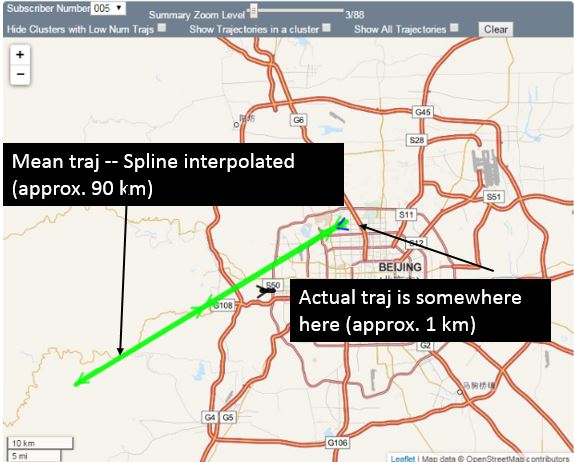
\includegraphics[scale=0.4]{figs/spline.jpg}
%\caption{Problems with spline interpolation}
%\label{fig:spline}
%\end{figure}
%\paragraph{Resampling and then applying DTW is very close to using our similarity measure }
%\end{comment}
